\documentclass{ximera}
%geschreven 9/11/26
\title{Vragen het magnetisch veld}
\author{Daan Lipkens}

\begin{document}
\begin{abstract}
    Conceptuele vragen over magneten, veldlijnen, rechterhandregels en elektromagneten.
\end{abstract}
\maketitle

\section{Conceptuele vragen het magnetisch veld}

%———————————————————————————————————————
% VRAAG 1: ferromagnetische stoffen
\begin{question}
    Welke voorwerpen worden door een magneet aangetrokken? Duid alle juiste antwoorden aan.

    \begin{selectAll}
        \choice[correct]{een ijzeren spijker}
        \choice{een koperen buisje}
        \choice[correct]{een stalen schaar}
        \choice{een gouden ring}
        \choice[correct]{een plaatje nikkel}
        \choice{een stuk aluminiumfolie}
    \end{selectAll}

    \begin{solution}\nl
        Enkel ferromagnetische stoffen worden aangetrokken: ijzer, kobalt, nikkel en legeringen zoals staal. Koper, goud en aluminium zijn niet ferromagnetisch.
    \end{solution}
\end{question}
%———————————————————————————————————————

%———————————————————————————————————————
% VRAAG 2: onbekende pool
\begin{question}
    Op een staafmagneet zijn de letters N en Z weggesleten. Je houdt een kompas bij uiteinde $A$ van de magneet en ziet dat de \textbf{noordpool} van de kompasnaald naar $A$ toe draait. Welke pool is $A$?

    \begin{multipleChoice}
        \choice{een noordpool}
        \choice[correct]{een zuidpool}
        \choice{dat kan je zo niet weten}
    \end{multipleChoice}

    \begin{solution}\nl
        De noordpool van de naald wordt aangetrokken door een ongelijknamige pool. Uiteinde $A$ is dus een zuidpool.
    \end{solution}
\end{question}
%———————————————————————————————————————

%———————————————————————————————————————
% VRAAG 3: veld bestaat zonder kompas
\begin{question}
    Een leerling zegt: \enquote{Het magnetisch veld in punt $P$ bestaat pas als je er een kompas neerlegt.} Heeft hij gelijk?

    \begin{multipleChoice}
        \choice{Ja, zonder kompas is er niets dat een kracht ondervindt.}
        \choice[correct]{Nee, het veld wordt gemaakt door de magneet. Het kompas toont het veld enkel aan.}
        \choice{Ja, het kompas maakt zelf het veld dat het meet.}
    \end{multipleChoice}

    \begin{solution}\nl
        Net als een testlading bij het elektrisch veld is een kompasnaald enkel een meetinstrument. Het magnetisch veld in $P$ wordt gemaakt door de magneet (of de stroom), ook als er geen kompas ligt.
    \end{solution}
\end{question}
%———————————————————————————————————————

%———————————————————————————————————————
% VRAAG 4: veldlijnendichtheid
\begin{question}
    De figuur toont enkele veldlijnen van een magnetisch veld. Waar is het veld het sterkst?

    \begin{center}
        \begin{tikzpicture}
            \foreach \a/\b in {1.5/0.6, 0.5/0.2, -0.5/-0.2, -1.5/-0.6}{
                \draw[Mveldlijn] (0,\a) .. controls (2,\a) and (3,\b) .. (5,\b);
            }
            \fill (0.6,1.0) circle (0.6mm) node[above]{$A$};
            \fill (2.5,-0.05) circle (0.6mm) node[below]{$B$};
            \fill (4.6,0.4) circle (0.6mm) node[above]{$C$};
        \end{tikzpicture}
    \end{center}

    \begin{multipleChoice}
        \choice{in $A$}
        \choice{in $B$}
        \choice[correct]{in $C$}
        \choice{overal even sterk}
    \end{multipleChoice}

    \begin{solution}\nl
        De veldlijnen komen naar rechts toe dichter bij elkaar. Waar de veldlijnen het dichtst liggen, is het veld het sterkst: in $C$.
    \end{solution}
\end{question}
%———————————————————————————————————————

%———————————————————————————————————————
% VRAAG 5: veld van een draad, stroom in het blad
\begin{question}
    Door een rechte draad loodrecht op het blad loopt een stroom \textbf{in het blad}. Punt $P$ ligt \textbf{onder} de draad. Welke zin heeft het magnetisch veld in $P$?

    \begin{center}
        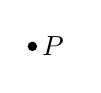
\begin{tikzpicture}
            \stroomin{D}{0,0}
            \fill (0,-1.2) circle (0.6mm) node[right]{$P$};
        \end{tikzpicture}
    \end{center}

    \begin{multipleChoice}
        \choice{naar boven, naar de draad toe}
        \choice{naar onder, weg van de draad}
        \choice[correct]{naar links}
        \choice{naar rechts}
    \end{multipleChoice}

    \begin{hint}
        Wijs met je rechterduim het blad in. In welke zin draaien je vingers? Welke kant wijst de raaklijn onderaan zo'n cirkel?
    \end{hint}

    \begin{solution}\nl
        Met de duim het blad in krullen de vingers in wijzerzin. Onderaan een cirkel in wijzerzin wijst de raaklijn naar links. Het veld staat steeds loodrecht op de verbindingslijn met de draad.
    \end{solution}
\end{question}
%———————————————————————————————————————

%———————————————————————————————————————
% VRAAG 6: pool van een spoel
\begin{question}
    Je kijkt in de opening van een spoel. Gezien vanuit jouw standpunt loopt de stroom in de windingen in \textbf{wijzerzin}. Welke pool van de spoel is naar jou gericht?

    \begin{multipleChoice}
        \choice{een noordpool}
        \choice[correct]{een zuidpool}
        \choice{geen van beide, een spoel heeft geen polen}
    \end{multipleChoice}

    \begin{hint}
        Krul de vingers van je rechterhand in wijzerzin. Waar wijst je duim naartoe: naar jou of van je weg?
    \end{hint}

    \begin{solution}\nl
        Met de vingers in wijzerzin wijst de duim van je weg. De veldlijnen in de spoel lopen dus van je weg: aan jouw kant gaan ze de spoel binnen. Waar de veldlijnen binnengaan, ligt de zuidpool.
    \end{solution}
\end{question}
%———————————————————————————————————————

%———————————————————————————————————————
% VRAAG 7: twee draden, zelfde zin
\begin{question}
    Twee evenwijdige draden voeren een even grote stroom in \textbf{dezelfde zin}. Hoe groot is het magnetisch veld in het punt precies midden tussen de draden?

    \begin{multipleChoice}
        \choice[correct]{nul}
        \choice{even groot als het veld van één draad}
        \choice{twee keer zo groot als het veld van één draad}
    \end{multipleChoice}

    \begin{hint}
        Teken een bovenaanzicht met beide stromen uit het blad en bepaal de zin van elk veld in het middelpunt.
    \end{hint}

    \begin{solution}\nl
        Beide velden zijn even groot, want de stromen en de afstanden zijn gelijk. Met beide stromen uit het blad wijst het veld van de linkse draad in het midden naar boven, dat van de rechtse draad naar onder. Ze heffen elkaar op.
    \end{solution}
\end{question}
%———————————————————————————————————————

%———————————————————————————————————————
% VRAAG 8: twee draden, tegengestelde zin
\begin{question}
    Twee evenwijdige draden voeren een even grote stroom in \textbf{tegengestelde zin}. Hoe groot is het magnetisch veld in het punt precies midden tussen de draden?

    \begin{multipleChoice}
        \choice{nul}
        \choice{even groot als het veld van één draad}
        \choice[correct]{twee keer zo groot als het veld van één draad}
    \end{multipleChoice}

    \begin{solution}\nl
        Keer je de stroom in één draad om, dan keert ook het veld van die draad om. In het midden wijzen beide velden nu dezelfde kant op en tellen ze op tot twee keer het veld van één draad.
    \end{solution}
\end{question}
%———————————————————————————————————————

%———————————————————————————————————————
% VRAAG 9: veld spoel, verband
\begin{question}
    Een spoel heeft $400$ windingen over een lengte van $20\,\mathrm{cm}$. Een tweede spoel heeft $200$ windingen over $10\,\mathrm{cm}$ en een twee keer grotere diameter. Door beide loopt dezelfde stroom. Hoe verhoudt het veld in de tweede spoel zich tot dat in de eerste?

    \begin{multipleChoice}
        \choice{half zo groot}
        \choice[correct]{even groot}
        \choice{twee keer zo groot}
        \choice{vier keer zo groot}
    \end{multipleChoice}

    \begin{solution}\nl
        Het veld in een spoel hangt af van de windingsdichtheid $N/\ell$ en de stroom, niet van de diameter. Beide spoelen hebben $2000$ windingen per meter: het veld is even groot.
    \end{solution}
\end{question}
%———————————————————————————————————————

%———————————————————————————————————————
% VRAAG 10: analogie
\begin{question}
    Welke uitspraak over het magnetisch veld en het elektrisch veld is juist?

    \begin{multipleChoice}
        \choice{Beide velden worden veroorzaakt door ladingen in rust.}
        \choice[correct]{Elektrische veldlijnen starten en eindigen op ladingen, magnetische veldlijnen vormen gesloten lussen.}
        \choice{Je kan een noordpool afzonderen, net zoals een positieve lading.}
        \choice{Magnetische veldlijnen kunnen elkaar snijden, elektrische niet.}
    \end{multipleChoice}

    \begin{solution}\nl
        Een elektrisch veld hoort bij ladingen, een magnetisch veld bij bewegende ladingen. Omdat er geen afzonderlijke magnetische polen bestaan, hebben magnetische veldlijnen geen begin of einde: ze vormen gesloten lussen. Geen enkel soort veldlijnen kan elkaar snijden.
    \end{solution}
\end{question}
%———————————————————————————————————————

%———————————————————————————————————————
% VRAAG 11: elektromagneet ompolen
\begin{question}
    Hoe wissel je de noordpool en de zuidpool van een elektromagneet om?

    \begin{multipleChoice}
        \choice{door de stroom te verdubbelen}
        \choice[correct]{door de zin van de stroom om te keren}
        \choice{door de weekijzeren kern te vervangen door een stalen kern}
        \choice{door de spoel langer te maken}
    \end{multipleChoice}

    \begin{solution}\nl
        De zin van het veld in een spoel volgt de stroomzin (rechterhandregel). Keer je de stroom om, dan keert ook het veld om en wisselen de polen.
    \end{solution}
\end{question}
%———————————————————————————————————————

%———————————————————————————————————————
% VRAAG 12: draad wikkelen
\begin{question}
    Je hebt een vaste lengte koperdraad en wil er een spoel mee maken met een zo groot mogelijk magnetisch veld bij dezelfde stroom. Op welke buis wikkel je de draad, telkens over de volledige lengte van de buis?

    \begin{multipleChoice}
        \choice{een lange, dikke buis}
        \choice{een lange, dunne buis}
        \choice{een korte, dikke buis}
        \choice[correct]{een korte, dunne buis}
    \end{multipleChoice}

    \begin{hint}
        Waar krijg je met dezelfde draad de meeste windingen? En waarvan hangt het veld in de spoel af?
    \end{hint}

    \begin{solution}\nl
        Op een dunne buis is elke winding korter, dus krijg je met dezelfde draad meer windingen $N$. Op een korte buis is $\ell$ klein. Beide maken de windingsdichtheid $N/\ell$ en dus het veld $B = \mu_0 \cdot N \cdot I/\ell$ zo groot mogelijk.
    \end{solution}
\end{question}
%———————————————————————————————————————

\end{document}
